\documentclass[11pt, a4paper]{article}

\usepackage[T1]{fontenc}
\usepackage[utf8]{inputenc}
\usepackage[polish]{babel}
\usepackage{listings}
\usepackage{mathtools}
\usepackage{blindtext}
\usepackage{scrextend}
\usepackage{graphicx}


\graphicspath{ {./images/} }


\begin{document}

\title{MOwNiT\\Laboratorium 2}
\author{Kacper Janda}
\date{}
\maketitle

\section{Porównanie algorytmów mnożenia macierzy}
Mnożenie macierzy kwadratowych:
\begin{center}
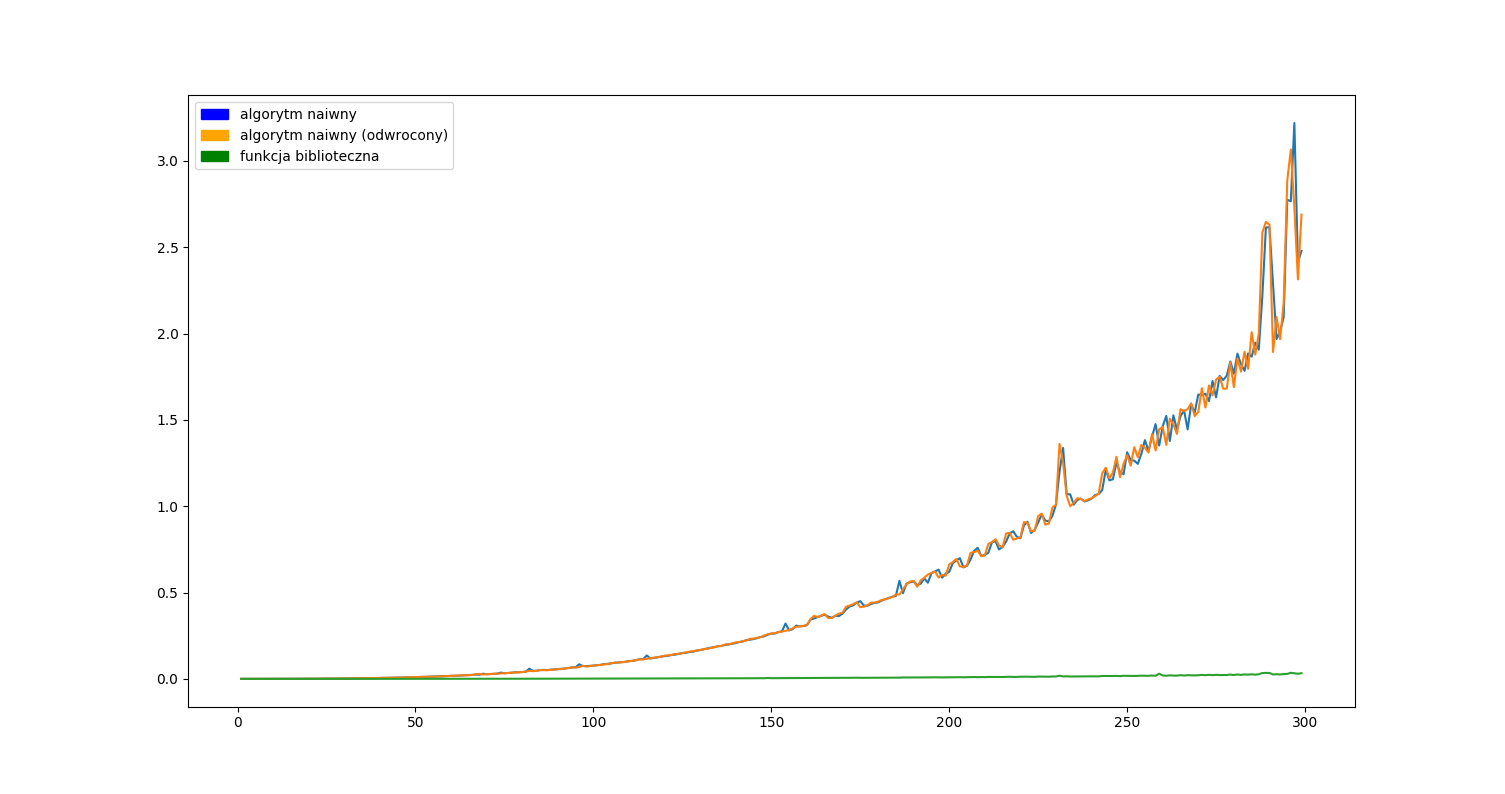
\includegraphics[scale = 0.32]{f1}
\end{center}

Mnożenie macierzy prostokątnych - na osi odciętych znajdują się wartości jednego z wymiarów macierzy - drugi jest \begin{math} 1000 \end{math} razy większy
\begin{center}
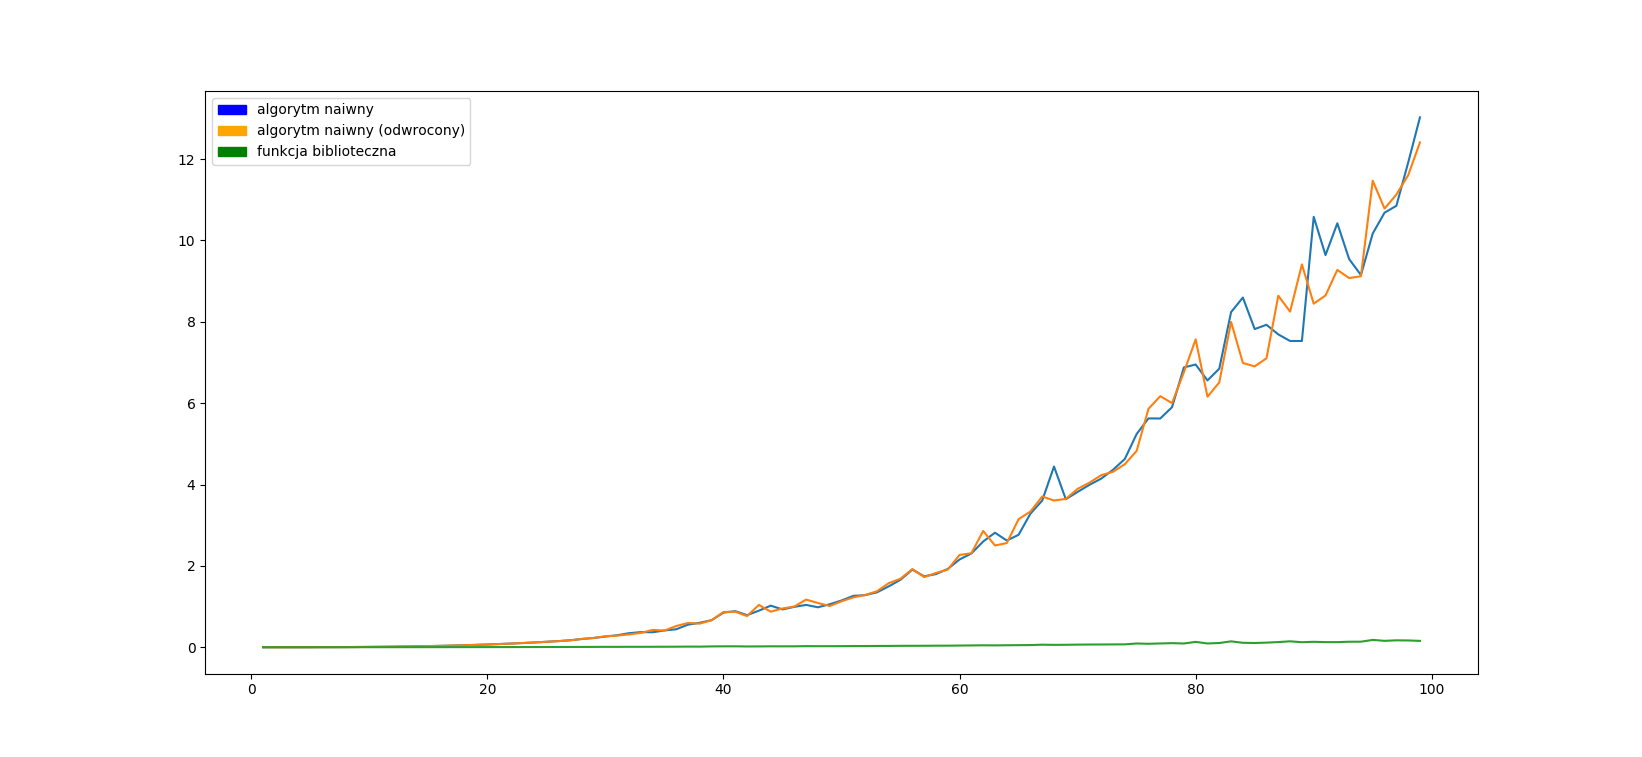
\includegraphics[scale = 0.32]{f2}
\end{center}
Do wykonania obliczeń został wykorzystany język Python oraz biblioteka numeryczna Numpy. Z wykresów wynika, że w tym języku nie jest istotna kolejność zagnieżdżenia pętli. Przeciwne zachowanie występuje na przykład w języku C czy Octave.

\end{document}